\documentclass[svgnames, tikz]{standalone}


\usepackage{tikz}
\usepackage{tikz-3dplot}
\usepackage{amsmath} %математические формулы
\usepackage[e]{esvect}  %Красивая стрелочка вектора
\usepackage{unicode-math}


\usepackage{polyglossia}
\setdefaultlanguage{russian}
\setotherlanguage{english}
%\setkeys{russian}{babelshorthands=true}
\usepackage{fontspec}
\setmainfont{Times New Roman} [Script=Cyrillic, Mapping=tex-text,]
\setsansfont{Arial} [Script=Cyrillic, Mapping=tex-text,]
\setmonofont{Courier New} [Script=Cyrillic, Mapping=tex-text,]

\usetikzlibrary{calc}
\usetikzlibrary{arrows.meta}
\usetikzlibrary{angles}




\usepackage{pgfmath}

\newcommand{\VARPOINT}[4] 
{
	
	\expandafter\edef\csname #1x\endcsname{\fpeval{#2}}
	\expandafter\edef\csname #1y\endcsname{\fpeval{#3}}
	\expandafter\edef\csname #1z\endcsname{\fpeval{#4}}
	
	\coordinate (#1) at (\csname #1x\endcsname,\csname #1y\endcsname,\csname #1z\endcsname );
	\coordinate (#1xy) at (\csname #1x\endcsname ,\csname #1y\endcsname ,0);
	\coordinate (#1xz) at (\csname #1x\endcsname ,0,\csname #1z\endcsname );
	\coordinate (#1yz) at (0,\csname #1y\endcsname ,\csname #1z\endcsname );
	\coordinate (#1x) at (\csname #1x\endcsname ,0, 0);
	\coordinate (#1y) at (0, \csname #1y\endcsname ,0);
	\coordinate (#1z) at (0, 0, \csname #1z\endcsname );
	
	%\FPeval{\x}{#2}
	%\FPeval{\y}{#3}
	%\FPeval{\z}{#4}		
	

	
}

\newcommand{\VECTOR}[2]
{
	
	\FPset{\x}{0}
	\FPset{\y}{0}
	\FPset{\z}{0}
	\FPsub{\x}{\csname #2x\endcsname}{\csname #1x\endcsname}
	\FPsub{\y}{\csname #2y\endcsname}{\csname #1y\endcsname}
	\FPsub{\z}{\csname #2z\endcsname}{\csname #1z\endcsname}
	
	
	%\expandafter\VARPOINT {vec#1#2}{\csname #1x}{0}{0}
	\expandafter\VARPOINT {vec#1#2}{\x}{\y}{\z}
}

\newcommand{\VIPI}[2]
{
	\def\tmpax{\csname #1x\endcsname}
	\def\tmpay{\csname #1y\endcsname}
	\def\tmpaz{\csname #1z\endcsname}
	
	\def\tmpbx{\csname #2x\endcsname}
	\def\tmpby{\csname #2y\endcsname}
	\def\tmpbz{\csname #2z\endcsname}
	
	\FPeval{\resultx}{\tmpay * \tmpbz - \tmpaz * \tmpby}
	\FPeval{\resulty}{\tmpaz * \tmpbx - \tmpax * \tmpbz}
	\FPeval{\resultz}{\tmpax * \tmpby - \tmpay * \tmpbx}
	
	\expandafter\VARPOINT {vp#1#2}{\resultx}{\resulty}{\resultz}	
	
}


\newcommand{\CALCZ}[4]{ %1-точка 2-n 3c 4-ответ
	
	\edef\tmpx{\csname #1x\endcsname}
	\edef\tmpy{\csname #1y\endcsname}	
	\edef\tmpnx{\csname #2x\endcsname}
	\edef\tmpny{\csname #2y\endcsname}
	\edef\tmpnz{\csname #2z\endcsname}
	\expandafter\edef\noexpand #4{\fpeval{( #3 - \tmpx * \tmpnx - \tmpy * \tmpny ) /  \tmpnz }}	
	\csname #4\endcsname
}



\newcommand{\dotsize}{1pt}
\newcommand{\PROJECTILELINES}[3] %1 -точка, 2 - стиль линий, 3 стиль кругов
{
	\draw [#2]  (#1z) -- (#1yz) -- (#1y) -- (#1xy) -- (#1x) -- (#1xz) -- cycle;
	\draw [#2]  (#1) -- (#1xy);     
	\draw [#2]  (#1) -- (#1yz); 
	\draw [#2]  (#1) -- (#1xz); 
	
	\fill [#3] (#1xy) circle [radius=\dotsize];
	\fill [#3] (#1yz) circle [radius=\dotsize];
	\fill [#3] (#1xz) circle [radius=\dotsize];
}

\newcommand{\PROJECTILELINESXY}[3] %1 -точка, 2 - стиль линий, 3 стиль кругов
{
	\draw [#2]  (#1) -- (#1xy);     		
	\fill [#3] (#1xy) circle [radius=\dotsize];	
}

\newcommand{\ROTATE}[3] %1-точка, 2 - ось, 3 - угол
{
	\expandafter\edef\csname tmpcosfi\endcsname{\fpeval{cos(#3)}}
	\expandafter\edef\csname tmpsinfi\endcsname{\fpeval{sin(#3)}}
	\expandafter\edef\csname tmpx\endcsname{\csname #1x\endcsname}
	\expandafter\edef\csname tmpy\endcsname{\csname #1y\endcsname}
	\expandafter\edef\csname tmpz\endcsname{\csname #1z\endcsname}
	
	\expandafter\edef\csname tmpOx\endcsname{\csname #2x\endcsname}
	\expandafter\edef\csname tmpOy\endcsname{\csname #2y\endcsname}
	\expandafter\edef\csname tmpOz\endcsname{\csname #2z\endcsname}
%	
	\expandafter\edef\csname tmplen\endcsname{\fpeval{ sqrt(\tmpOx*\tmpOx + \tmpOy*\tmpOy + \tmpOz*\tmpOz)  }}
%	
	\expandafter\edef\csname tmpOx\endcsname{\fpeval{\tmpOx / \tmplen}}
	\expandafter\edef\csname tmpOy\endcsname{\fpeval{\tmpOy / \tmplen}}
	\expandafter\edef\csname tmpOz\endcsname{\fpeval{\tmpOz / \tmplen}}
%	
	
	
	
%	
	\expandafter\edef\csname tmpAA\endcsname{\fpeval{ \tmpcosfi + (1-\tmpcosfi)*\tmpOx*\tmpOx  }}
	\expandafter\edef\csname tmpAB\endcsname{\fpeval{ (1-\tmpcosfi)*\tmpOx*\tmpOy - \tmpsinfi*\tmpOz  }}
	\expandafter\edef\csname tmpAC\endcsname{\fpeval{ (1-\tmpcosfi)*\tmpOx*\tmpOz + \tmpsinfi*\tmpOy   }}
	
	\expandafter\edef\csname tmpBA\endcsname{\fpeval{ (1-\tmpcosfi)*\tmpOx*\tmpOy + \tmpsinfi*\tmpOz  }}
	\expandafter\edef\csname tmpBB\endcsname{\fpeval{ \tmpcosfi + (1-\tmpcosfi)*\tmpOy*\tmpOy  }}
	\expandafter\edef\csname tmpBC\endcsname{\fpeval{ (1-\tmpcosfi)*\tmpOy*\tmpOz - \tmpsinfi*\tmpOx  }}
	
	\expandafter\edef\csname tmpCA\endcsname{\fpeval{ (1-\tmpcosfi)*\tmpOz*\tmpOx - \tmpsinfi*\tmpOy  }}
	\expandafter\edef\csname tmpCB\endcsname{\fpeval{ (1-\tmpcosfi)*\tmpOz*\tmpOy + \tmpsinfi*\tmpOx   }}
	\expandafter\edef\csname tmpCC\endcsname{\fpeval{ \tmpcosfi + (1-\tmpcosfi)*\tmpOz*\tmpOz  }}
	
	
	\expandafter\edef\csname tmpOutx\endcsname{\fpeval{  \tmpAA*\tmpx + \tmpAB*\tmpy + \tmpAC*\tmpz }}
	\expandafter\edef\csname tmpOuty\endcsname{\fpeval{  \tmpBA*\tmpx + \tmpBB*\tmpy + \tmpBC*\tmpz }}
	\expandafter\edef\csname tmpOutz\endcsname{\fpeval{  \tmpCA*\tmpx + \tmpCB*\tmpy + \tmpCC*\tmpz }}
	
	
	\VARPOINT{#1}{\tmpOutx}{\tmpOuty}{\tmpOutz}
	
}

\newcommand{\ROTATEPLANAR}[2]
{
	\expandafter\edef\noexpand\tmpx{\csname #1x\endcsname}
	\expandafter\edef\noexpand\tmpy{\csname #1y\endcsname}
	\expandafter\edef\noexpand\tmpz{\csname #1z\endcsname}
	
	\expandafter\edef\noexpand\tmpcosfi{\fpeval{cos(#2)}}
	\expandafter\edef\noexpand\tmpsinfi{\fpeval{sin(#2)}}
	
	\expandafter\edef\noexpand\tmpnewx{\fpeval{ \tmpcosfi * \tmpx - \tmpsinfi * \tmpy  }}
	\expandafter\edef\noexpand\tmpnewy{\fpeval{ \tmpsinfi * \tmpx + \tmpcosfi * \tmpy  }}
	
	\VARPOINT{#1}{\tmpnewx}{\tmpnewy}{\tmpz}
}

\begin{document}
	
    
 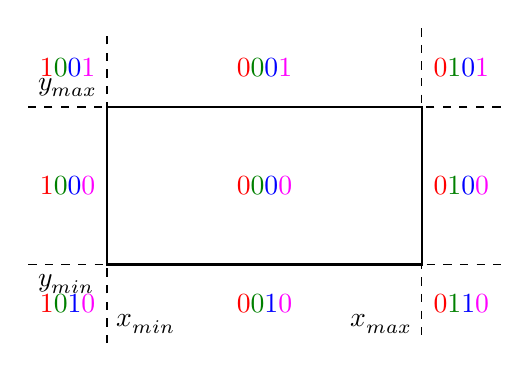
\begin{tikzpicture}[ scale=0.5]
	
	
	
	\VARPOINT{A}{-4}{-2}{0}
	\VARPOINT{B}{4}{-2}{0}
	\VARPOINT{C}{4}{2}{0}
	\VARPOINT{D}{-4}{2}{0}
	
	
	\draw[dashed] ($(A)!-2cm!(B)$) node [below right]{$y_{min}$} -- ($(B)!-2cm!(A)$);
	\draw[dashed] ($(C)!-2cm!(D)$)  -- ($(D)!-2cm!(C)$) node [above right]{$y_{max}$};
	
	\draw[dashed] ($(A)!-2cm!(D)$) node [above right]{$x_{min}$} -- ($(D)!-2cm!(A)$);
	\draw[dashed] ($(C)!-2cm!(B)$) -- ($(B)!-2cm!(C)$) node [above left]{$x_{max}$};
	
	\draw[thick] (A) -- (B) -- (C) -- (D) --cycle;
	
	
	
	\node at (-5,	-3) 	{ {\color{Red}1}{\color{Green}0}{\color{Blue}1}{\color{Fuchsia}0}};
	\node at (-5,	0) 		{ {\color{Red}1}{\color{Green}0}{\color{Blue}0}{\color{Fuchsia}0}};
	\node at (-5,	3) 		{ {\color{Red}1}{\color{Green}0}{\color{Blue}0}{\color{Fuchsia}1}};
	
	\node at (0,	-3) 	{ {\color{Red}0}{\color{Green}0}{\color{Blue}1}{\color{Fuchsia}0}};
	\node at (0,	0) 		{ {\color{Red}0}{\color{Green}0}{\color{Blue}0}{\color{Fuchsia}0}};
	\node at (0,	3) 		{ {\color{Red}0}{\color{Green}0}{\color{Blue}0}{\color{Fuchsia}1}};
	
	\node at (5,	-3) 	{ {\color{Red}0}{\color{Green}1}{\color{Blue}1}{\color{Fuchsia}0}};
	\node at (5,	0) 		{ {\color{Red}0}{\color{Green}1}{\color{Blue}0}{\color{Fuchsia}0}};
	\node at (5,	3) 		{ {\color{Red}0}{\color{Green}1}{\color{Blue}0}{\color{Fuchsia}1}};
	
	
	
\end{tikzpicture} 


 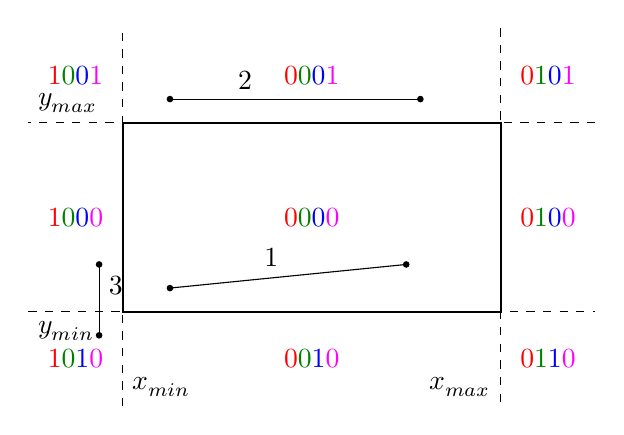
\begin{tikzpicture}[ scale=0.6]
	
	
	
	\VARPOINT{A}{-4}{-2}{0}
	\VARPOINT{B}{4}{-2}{0}
	\VARPOINT{C}{4}{2}{0}
	\VARPOINT{D}{-4}{2}{0}
	
	
	\draw[dashed] ($(A)!-2cm!(B)$) node [below right]{$y_{min}$} -- ($(B)!-2cm!(A)$);
	\draw[dashed] ($(C)!-2cm!(D)$)  -- ($(D)!-2cm!(C)$) node [above right]{$y_{max}$};
	
	\draw[dashed] ($(A)!-2cm!(D)$) node [above right]{$x_{min}$} -- ($(D)!-2cm!(A)$);
	\draw[dashed] ($(C)!-2cm!(B)$) -- ($(B)!-2cm!(C)$) node [above left]{$x_{max}$};
	
	\draw[thick] (A) -- (B) -- (C) -- (D) --cycle;
	
	
	
	\node at (-5,	-3) 	{ {\color{Red}1}{\color{Green}0}{\color{Blue}1}{\color{Fuchsia}0}};
\node at (-5,	0) 		{ {\color{Red}1}{\color{Green}0}{\color{Blue}0}{\color{Fuchsia}0}};
\node at (-5,	3) 		{ {\color{Red}1}{\color{Green}0}{\color{Blue}0}{\color{Fuchsia}1}};

\node at (0,	-3) 	{ {\color{Red}0}{\color{Green}0}{\color{Blue}1}{\color{Fuchsia}0}};
\node at (0,	0) 		{ {\color{Red}0}{\color{Green}0}{\color{Blue}0}{\color{Fuchsia}0}};
\node at (0,	3) 		{ {\color{Red}0}{\color{Green}0}{\color{Blue}0}{\color{Fuchsia}1}};

\node at (5,	-3) 	{ {\color{Red}0}{\color{Green}1}{\color{Blue}1}{\color{Fuchsia}0}};
\node at (5,	0) 		{ {\color{Red}0}{\color{Green}1}{\color{Blue}0}{\color{Fuchsia}0}};
\node at (5,	3) 		{ {\color{Red}0}{\color{Green}1}{\color{Blue}0}{\color{Fuchsia}1}};
	
	
	\VARPOINT{A1}{-3}{-1.5}{0}	
	\VARPOINT{B1}{2}{-1}{0}
	
	
	\path (A1) circle(2pt)[fill]  edge node[auto]{1} (B1)  (B1) circle (2pt)[fill];
	
	
	\VARPOINT{A1}{-3}{2.5}{0}	
	\VARPOINT{B1}{2.3}{2.5}{0}
	
	\path (A1) circle(2pt)[fill]  edge node[auto, pos=0.3]{2} (B1)  (B1) circle (2pt)[fill];
	
	
	
	\VARPOINT{A1}{-4.5}{-1}{0}	
	\VARPOINT{B1}{-4.5}{-2.5}{0}
	
	\path (A1) circle(2pt)[fill]  edge node[auto, pos=0.3]{3} (B1)  (B1) circle (2pt)[fill];
	
	
	
\end{tikzpicture} 




 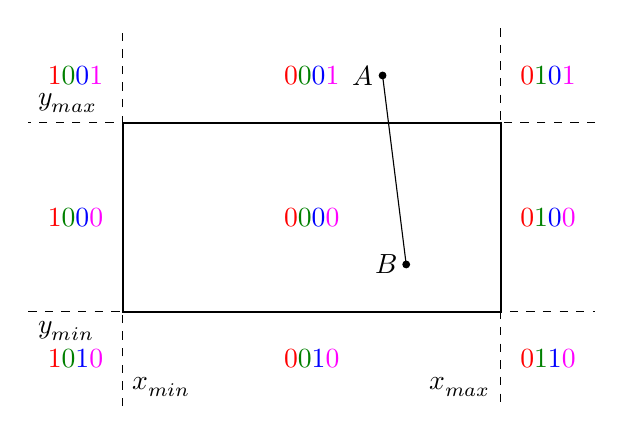
\begin{tikzpicture}[ scale=0.6]
	
	
	
	\VARPOINT{A}{-4}{-2}{0}
	\VARPOINT{B}{4}{-2}{0}
	\VARPOINT{C}{4}{2}{0}
	\VARPOINT{D}{-4}{2}{0}
	
	
	\draw[dashed] ($(A)!-2cm!(B)$) node [below right]{$y_{min}$} -- ($(B)!-2cm!(A)$);
	\draw[dashed] ($(C)!-2cm!(D)$)  -- ($(D)!-2cm!(C)$) node [above right]{$y_{max}$};
	
	\draw[dashed] ($(A)!-2cm!(D)$) node [above right]{$x_{min}$} -- ($(D)!-2cm!(A)$);
	\draw[dashed] ($(C)!-2cm!(B)$) -- ($(B)!-2cm!(C)$) node [above left]{$x_{max}$};
	
	\draw[thick] (A) -- (B) -- (C) -- (D) --cycle;
	
	
	
	\node at (-5,	-3) 	{ {\color{Red}1}{\color{Green}0}{\color{Blue}1}{\color{Fuchsia}0}};
	\node at (-5,	0) 		{ {\color{Red}1}{\color{Green}0}{\color{Blue}0}{\color{Fuchsia}0}};
	\node at (-5,	3) 		{ {\color{Red}1}{\color{Green}0}{\color{Blue}0}{\color{Fuchsia}1}};
	
	\node at (0,	-3) 	{ {\color{Red}0}{\color{Green}0}{\color{Blue}1}{\color{Fuchsia}0}};
	\node at (0,	0) 		{ {\color{Red}0}{\color{Green}0}{\color{Blue}0}{\color{Fuchsia}0}};
	\node at (0,	3) 		{ {\color{Red}0}{\color{Green}0}{\color{Blue}0}{\color{Fuchsia}1}};
	
	\node at (5,	-3) 	{ {\color{Red}0}{\color{Green}1}{\color{Blue}1}{\color{Fuchsia}0}};
	\node at (5,	0) 		{ {\color{Red}0}{\color{Green}1}{\color{Blue}0}{\color{Fuchsia}0}};
	\node at (5,	3) 		{ {\color{Red}0}{\color{Green}1}{\color{Blue}0}{\color{Fuchsia}1}};
	
	
	\VARPOINT{A1}{1.5}{3}{0}	
	\VARPOINT{B1}{2}{-1}{0}
	
	
	\draw (A1)  circle(2pt)[fill]  edge  (B1) node [left] {$A$} (B1) circle (2pt)[fill] node [left] {$B$};
	

	
	
	
	
\end{tikzpicture} 

 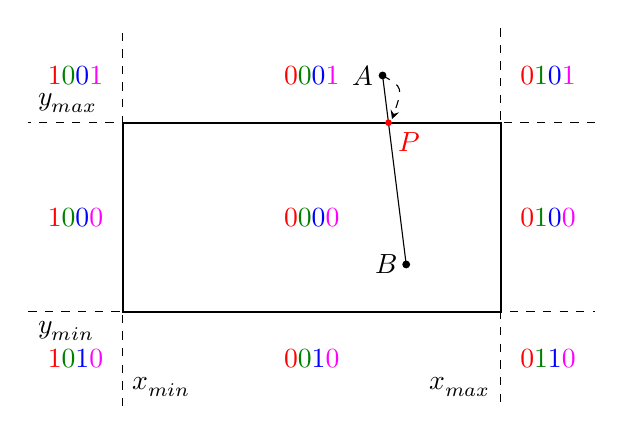
\begin{tikzpicture}[ scale=0.6]
	
	
	
	\VARPOINT{A}{-4}{-2}{0}
	\VARPOINT{B}{4}{-2}{0}
	\VARPOINT{C}{4}{2}{0}
	\VARPOINT{D}{-4}{2}{0}
	
	
	\draw[dashed] ($(A)!-2cm!(B)$) node [below right]{$y_{min}$} -- ($(B)!-2cm!(A)$);
	\draw[dashed] ($(C)!-2cm!(D)$)  -- ($(D)!-2cm!(C)$) node [above right]{$y_{max}$};
	
	\draw[dashed] ($(A)!-2cm!(D)$) node [above right]{$x_{min}$} -- ($(D)!-2cm!(A)$);
	\draw[dashed] ($(C)!-2cm!(B)$) -- ($(B)!-2cm!(C)$) node [above left]{$x_{max}$};
	
	\draw[thick] (A) -- (B) -- (C) -- (D) --cycle;
	
	
	
	\node at (-5,	-3) 	{ {\color{Red}1}{\color{Green}0}{\color{Blue}1}{\color{Fuchsia}0}};
	\node at (-5,	0) 		{ {\color{Red}1}{\color{Green}0}{\color{Blue}0}{\color{Fuchsia}0}};
	\node at (-5,	3) 		{ {\color{Red}1}{\color{Green}0}{\color{Blue}0}{\color{Fuchsia}1}};
	
	\node at (0,	-3) 	{ {\color{Red}0}{\color{Green}0}{\color{Blue}1}{\color{Fuchsia}0}};
	\node at (0,	0) 		{ {\color{Red}0}{\color{Green}0}{\color{Blue}0}{\color{Fuchsia}0}};
	\node at (0,	3) 		{ {\color{Red}0}{\color{Green}0}{\color{Blue}0}{\color{Fuchsia}1}};
	
	\node at (5,	-3) 	{ {\color{Red}0}{\color{Green}1}{\color{Blue}1}{\color{Fuchsia}0}};
	\node at (5,	0) 		{ {\color{Red}0}{\color{Green}1}{\color{Blue}0}{\color{Fuchsia}0}};
	\node at (5,	3) 		{ {\color{Red}0}{\color{Green}1}{\color{Blue}0}{\color{Fuchsia}1}};
	
	
	\VARPOINT{A1}{1.5}{3}{0}	
	\VARPOINT{B1}{2}{-1}{0}
	
	
	\draw (A1)  circle(2pt)[fill]  edge  (B1) node [left] {$A$} (B1) circle (2pt)[fill] node [left] {$B$};
	
	\coordinate (P) at (intersection of A1--B1 and D--C);
	
	\fill [red] (P) circle(2pt) node [below right] {$P$};
	
	\draw [-stealth, dashed] (A1) .. controls +(-30:0.5) .. ($(P)+(45:3pt)$);	

	
	
	
\end{tikzpicture} 


\foreach \frame in {1,2,3}{

 \begin{tikzpicture}[ scale=0.6]
	
	
	
	\VARPOINT{A}{-4}{-2}{0}
	\VARPOINT{B}{4}{-2}{0}
	\VARPOINT{C}{4}{2}{0}
	\VARPOINT{D}{-4}{2}{0}
	
	
	\draw[dashed] ($(A)!-2cm!(B)$) node [below right]{$y_{min}$} -- ($(B)!-2cm!(A)$);
	\draw[dashed] ($(C)!-2cm!(D)$)  -- ($(D)!-2cm!(C)$) node [above right]{$y_{max}$};
	
	\draw[dashed] ($(A)!-2cm!(D)$) node [above right]{$x_{min}$} -- ($(D)!-2cm!(A)$);
	\draw[dashed] ($(C)!-2cm!(B)$) -- ($(B)!-2cm!(C)$) node [above left]{$x_{max}$};
	
	\draw[thick] (A) -- (B) -- (C) -- (D) --cycle;
	
	
	
	\node at (-5,	-3) 	{ {\color{Red}1}{\color{Green}0}{\color{Blue}1}{\color{Fuchsia}0}};
	\node at (-5,	0) 		{ {\color{Red}1}{\color{Green}0}{\color{Blue}0}{\color{Fuchsia}0}};
	\node at (-5,	3) 		{ {\color{Red}1}{\color{Green}0}{\color{Blue}0}{\color{Fuchsia}1}};
	
	\node at (0,	-3) 	{ {\color{Red}0}{\color{Green}0}{\color{Blue}1}{\color{Fuchsia}0}};
	\node at (0,	0) 		{ {\color{Red}0}{\color{Green}0}{\color{Blue}0}{\color{Fuchsia}0}};
	\node at (0,	3) 		{ {\color{Red}0}{\color{Green}0}{\color{Blue}0}{\color{Fuchsia}1}};
	
	\node at (5,	-3) 	{ {\color{Red}0}{\color{Green}1}{\color{Blue}1}{\color{Fuchsia}0}};
	\node at (5,	0) 		{ {\color{Red}0}{\color{Green}1}{\color{Blue}0}{\color{Fuchsia}0}};
	\node at (5,	3) 		{ {\color{Red}0}{\color{Green}1}{\color{Blue}0}{\color{Fuchsia}1}};
	
	
	\VARPOINT{A1}{5}{2.5}{0}	
	\VARPOINT{B1}{1.7}{-3.3}{0}
	
	
	\draw (A1)  circle(2pt)[fill]  edge  (B1) node  [right] (a) {$A$} (B1) circle (2pt)[fill] node [left] (b) {$B$};
	
	
	

	\ifthenelse{\frame>1}{
		\coordinate (AA) at (intersection of A1--B1 and B--C);
		\fill[red] (AA) circle(2pt) node [right] (aa) {$A_1$};
		
		\draw [dashed, -stealth] (a) -- (aa);
	}{	}
	
	
	\ifthenelse{\frame>2}{
	
	\coordinate (BB) at (intersection of A1--B1 and B--A);
	
	\fill[red] (BB) circle(2pt) node [above left] (bb) {$B_1$};
	
	\draw[dashed, -stealth] (b) -- (bb);
	
	}{}
	
	
	
\end{tikzpicture} 

}



\foreach \frame in {1,2}{
	
	\begin{tikzpicture}[ scale=0.6]
		
		\clip (-7,-5) rectangle + (9,10);
		
		
		\VARPOINT{A}{-4}{-2}{0}
		\VARPOINT{B}{4}{-2}{0}
		\VARPOINT{C}{4}{2}{0}
		\VARPOINT{D}{-4}{2}{0}
		
		
		\draw[dashed] ($(A)!-2cm!(B)$)  -- ($(B)!-2cm!(A)$);
		\draw[dashed] ($(C)!-2cm!(D)$)  -- ($(D)!-2cm!(C)$) ;
		
		\draw[dashed] ($(A)!-2cm!(D)$)  -- ($(D)!-2cm!(A)$);
		\draw[dashed] ($(C)!-2cm!(B)$) -- ($(B)!-2cm!(C)$) ;
		
		\draw[thick] (A) -- (B) -- (C) -- (D) --cycle;
		
		
		
		\node at (-5,	-3) 	{ {\color{Red}1}{\color{Green}0}{\color{Blue}1}{\color{Fuchsia}0}};
		\node at (-5,	0) 		{ {\color{Red}1}{\color{Green}0}{\color{Blue}0}{\color{Fuchsia}0}};
		\node at (-5,	3) 		{ {\color{Red}1}{\color{Green}0}{\color{Blue}0}{\color{Fuchsia}1}};
		
		\node at (0,	-3) 	{ {\color{Red}0}{\color{Green}0}{\color{Blue}1}{\color{Fuchsia}0}};
		\node at (0,	0) 		{ {\color{Red}0}{\color{Green}0}{\color{Blue}0}{\color{Fuchsia}0}};
		\node at (0,	3) 		{ {\color{Red}0}{\color{Green}0}{\color{Blue}0}{\color{Fuchsia}1}};
		
		\node at (5,	-3) 	{ {\color{Red}0}{\color{Green}1}{\color{Blue}1}{\color{Fuchsia}0}};
		\node at (5,	0) 		{ {\color{Red}0}{\color{Green}1}{\color{Blue}0}{\color{Fuchsia}0}};
		\node at (5,	3) 		{ {\color{Red}0}{\color{Green}1}{\color{Blue}0}{\color{Fuchsia}1}};
		
		
		\VARPOINT{A1}{-3.5}{-4}{0}	
		\VARPOINT{B1}{-6}{2.5}{0}
		
		
		\draw (A1)  circle(2pt)[fill]  edge  (B1) node  [left] (a) {$A$} (B1) circle (2pt)[fill] node [left] (b) {$B$};
		
		
		
		
		\ifthenelse{\frame>1}{
			\coordinate (AA) at (intersection of A1--B1 and A--B);
			\fill[red] (AA) circle(2pt) node [above left] (aa) {$A_1$};
			
			\draw [dashed, -stealth] (a) -- (aa);
		}{	}
		
		
		\ifthenelse{\frame>2}{
			
			\coordinate (BB) at (intersection of A1--B1 and B--A);
			
			%\fill[red] (BB) circle(2pt) node [above left] (bb) {$B_1$};
			
			%\draw[dashed, ->] (b) -- (bb);
			
		}{}
		
		
		
	\end{tikzpicture} 
	
}




\foreach \frame in {1,2,3,4}{
	
	\begin{tikzpicture}[ scale=0.6]
		
		\clip (-7,-5) rectangle + (9,10);
		
		
		\VARPOINT{A}{-4}{-2}{0}
		\VARPOINT{B}{4}{-2}{0}
		\VARPOINT{C}{4}{2}{0}
		\VARPOINT{D}{-4}{2}{0}
		
		
		\draw[dashed] ($(A)!-2cm!(B)$)  -- ($(B)!-2cm!(A)$);
		\draw[dashed] ($(C)!-2cm!(D)$)  -- ($(D)!-2cm!(C)$) ;
		
		\draw[dashed] ($(A)!-2cm!(D)$)  -- ($(D)!-2cm!(A)$);
		\draw[dashed] ($(C)!-2cm!(B)$) -- ($(B)!-2cm!(C)$) ;
		
		\draw[thick] (A) -- (B) -- (C) -- (D) --cycle;
		
		
		
		\node at (-5,	-3) 	{ {\color{Red}1}{\color{Green}0}{\color{Blue}1}{\color{Fuchsia}0}};
		\node at (-5,	0) 		{ {\color{Red}1}{\color{Green}0}{\color{Blue}0}{\color{Fuchsia}0}};
		\node at (-5,	3) 		{ {\color{Red}1}{\color{Green}0}{\color{Blue}0}{\color{Fuchsia}1}};
		
		\node at (0,	-3) 	{ {\color{Red}0}{\color{Green}0}{\color{Blue}1}{\color{Fuchsia}0}};
		\node at (0,	0) 		{ {\color{Red}0}{\color{Green}0}{\color{Blue}0}{\color{Fuchsia}0}};
		\node at (0,	3) 		{ {\color{Red}0}{\color{Green}0}{\color{Blue}0}{\color{Fuchsia}1}};
		
		\node at (5,	-3) 	{ {\color{Red}0}{\color{Green}1}{\color{Blue}1}{\color{Fuchsia}0}};
		\node at (5,	0) 		{ {\color{Red}0}{\color{Green}1}{\color{Blue}0}{\color{Fuchsia}0}};
		\node at (5,	3) 		{ {\color{Red}0}{\color{Green}1}{\color{Blue}0}{\color{Fuchsia}1}};
		
		
		\VARPOINT{A1}{-4.3}{-4}{0}	
		\VARPOINT{B1}{-2}{3}{0}
		
		
		\draw (A1)  circle(2pt)[fill]  edge  (B1) node  [below right] (a) {$A$} (B1) circle (2pt)[fill] node [left] (b) {$B$};
		
		
		
		
		\ifthenelse{\frame>1}{
			\coordinate (AA) at (intersection of A1--B1 and A--D);
			\fill[red] (AA) circle(2pt) node [right] (aa) {$A_1$};
			
			\draw [dashed, -stealth] (a) -- (aa);
		}{	}
		
		
		\ifthenelse{\frame>2}{
			
			\coordinate (AA) at (intersection of A1--B1 and A--B);
			\fill[red] (AA) circle(2pt) node [above right] (aaa) {$A_2$};
			
			\draw [dashed, -stealth] (aa) -- (aaa);
			
			%\fill[red] (BB) circle(2pt) node [above left] (bb) {$B_1$};
			
			%\draw[dashed, ->] (b) -- (bb);
			
		}{}
		
		\ifthenelse{\frame>3}{
			
			\coordinate (AA) at (intersection of A1--B1 and C--D);
			\fill[red] (AA) circle(2pt) node [below left] (bb) {$B_1$};
			
			%\fill[red] (BB) circle(2pt) node [above left] (bb) {$B_1$};
			
			\draw[dashed, -stealth] (b) -- (bb);
			
		}{}
		
		
		
	\end{tikzpicture} 
	
}



    
   


	
\end{document}